\documentclass[tikz, border = 20pt]{standalone}
\usepackage[utf8]{inputenc}
\usepackage[english]{babel}
\usepackage{amsmath}
\usepackage{amsfonts}
\usepackage{amssymb}
\usepackage{graphicx}
\usepackage{lmodern}
\usepackage[left=3cm,right=2cm,top=2cm,bottom=2cm]{geometry}

	\usetikzlibrary{calc}
	\usetikzlibrary{shapes}
	\usetikzlibrary{arrows}
\begin{document}

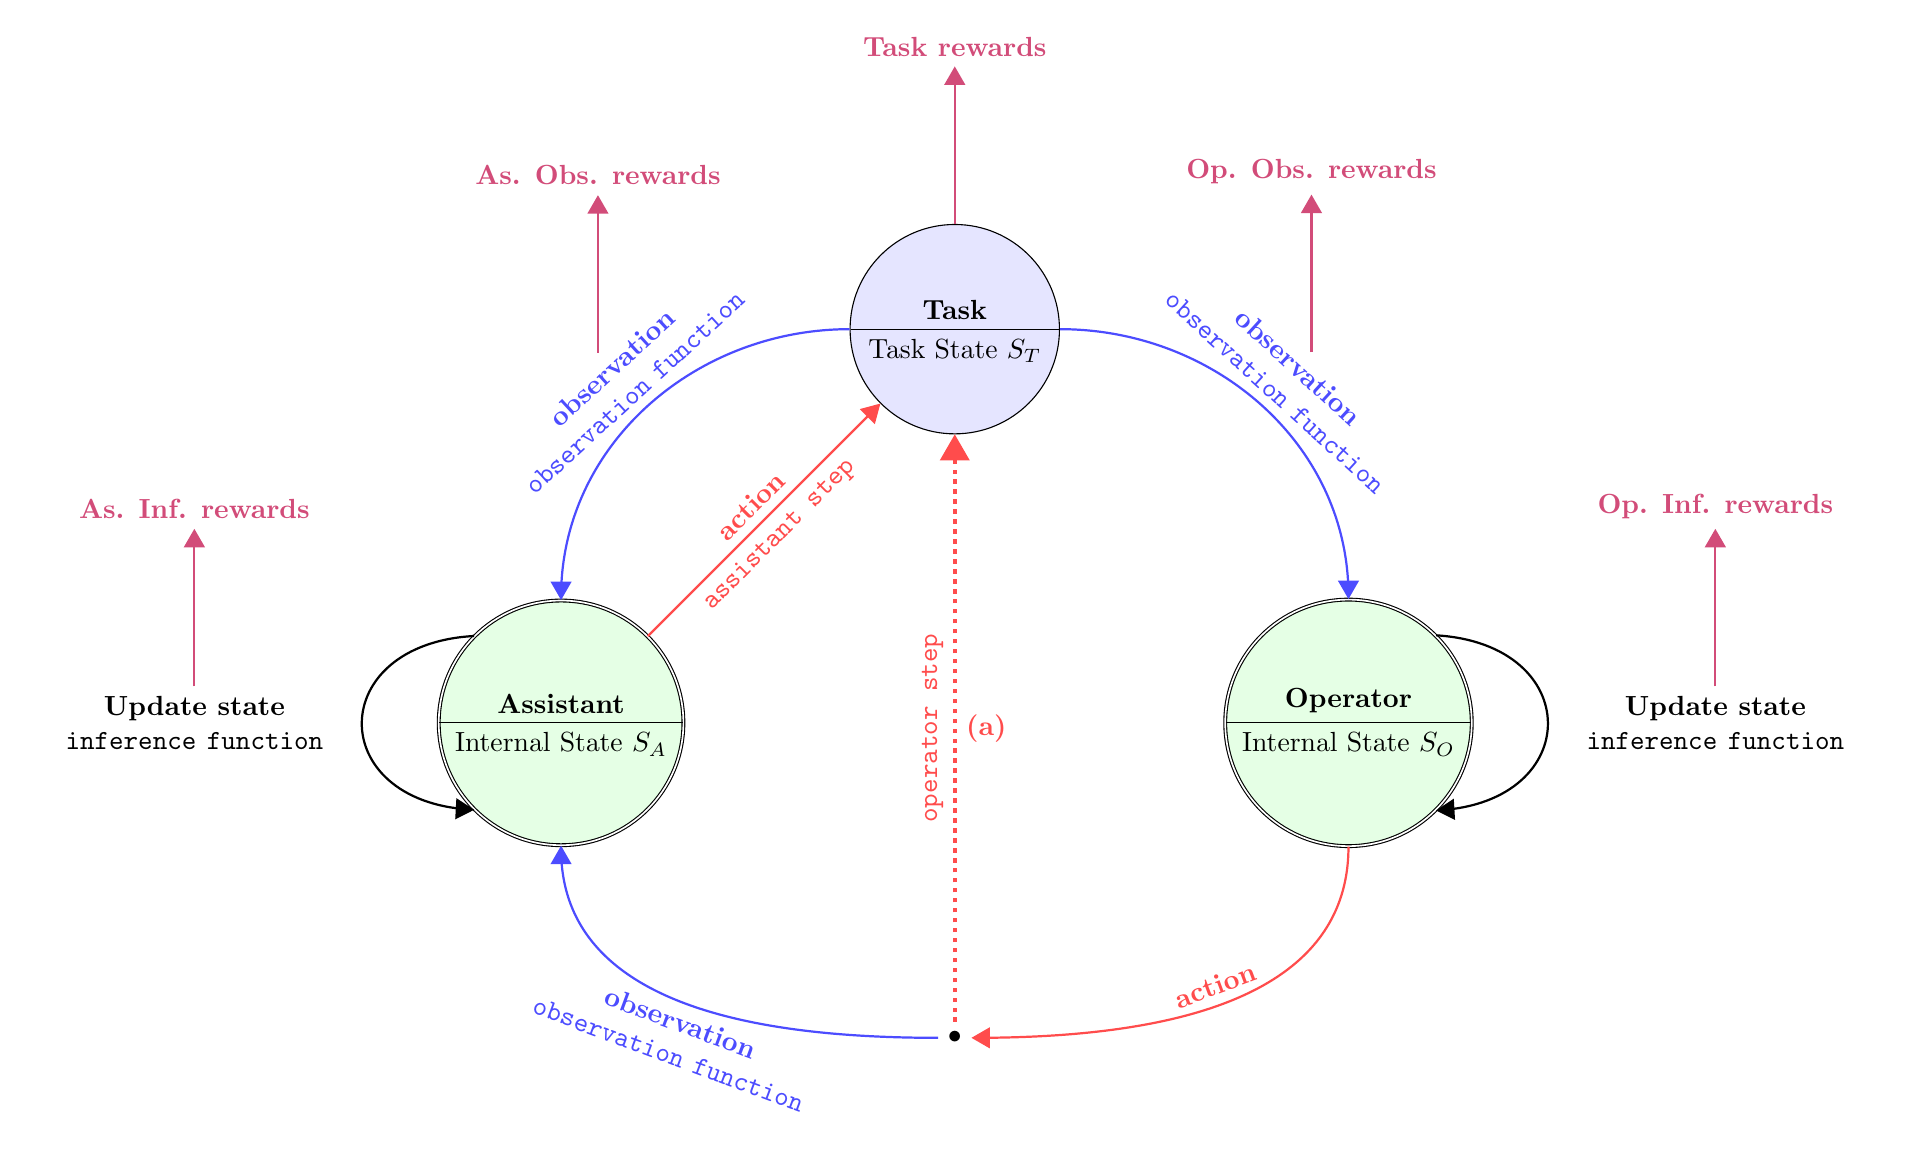
\begin{tikzpicture}
	\tikzstyle{every text node part}=[font=\bfseries]
	\tikzset{agent/.style = {circle split, draw, double, fill = green!10}}

%% Task node

\draw (0,0) node[name = task, circle split, draw, fill = blue!10]{Task \nodepart{lower}{Task State $S_T$}};
	
%% Operator Node
\draw (5,-5) node[agent, name = operator]{
	Operator
	\nodepart{lower}{Internal State $S_O$}	
	};
	
%% Invis node
\draw (0,-9) node[name = null]{$\bullet$};

	
%% assistant Node
\draw (-5,-5) node[agent, name = assistant]{
	Assistant
	\nodepart{lower}{Internal State $S_A$}	
	};
	
%% Edges
\draw[-triangle 60, thick, blue!70] (task.0) to[out = 0, in = 90] node[midway, sloped, above, text width = 4cm, text centered](label1){observation \texttt{observation~function}}(operator.90);

\draw[thick, -triangle 60, red!70] (operator.270) to[out = 270, in = 0] node[midway, sloped, above]{action} (null.0);
\draw[-triangle 60, dotted, ultra thick, red!70] (null) -- node[midway, right]{(a)} node[midway, rotate = 90, above]{\texttt{operator step}} (task.270);
\draw[-triangle 60, thick, blue!70] (null) to[out = 180, in = 270] node[midway, sloped, below, text width = 4cm, text centered](label3){observation \texttt{observation~function}} (assistant.270);
\draw[-triangle 60, thick, blue!70] (task.180) to[out = 180, in = 90] node[midway, sloped, above, text width = 4cm, text centered](label4){observation \texttt{observation~function}} (assistant.90);
\draw[-triangle 60, thick, red!70] (assistant.45) -- node[midway, above, sloped]{action} node[midway, below, sloped]{\texttt{assistant step}} (task.225);
\draw[-triangle 60, thick] (operator.45) .. controls (8,-4) and (8,-6).. node[midway, right, text width = 4cm, text centered](label2){Update state \texttt{inference~function}} (operator.315);
\draw[-triangle 60, thick] (assistant.135) .. controls (-8,-4) and (-8,-6).. node[midway, left, text width = 4cm, text centered](label5){Update state \texttt{inference~function}} (assistant.225);

\draw[-triangle 60, thick, purple!70] (task.90) -- +(0,2) node[above]{Task rewards};
\draw[-triangle 60, thick, purple!70] (label1.90) -- +(0,2) node[above]{Op. Obs. rewards};
\draw[-triangle 60, thick, purple!70] (label2.90) -- +(0,2) node[above]{Op. Inf. rewards};
\draw[-triangle 60, thick, purple!70] (label4.90) -- +(0,2) node[above]{As. Obs. rewards};
\draw[-triangle 60, thick, purple!70] (label5.90) -- +(0,2) node[above]{As. Inf. rewards};

\end{tikzpicture}



\end{document}